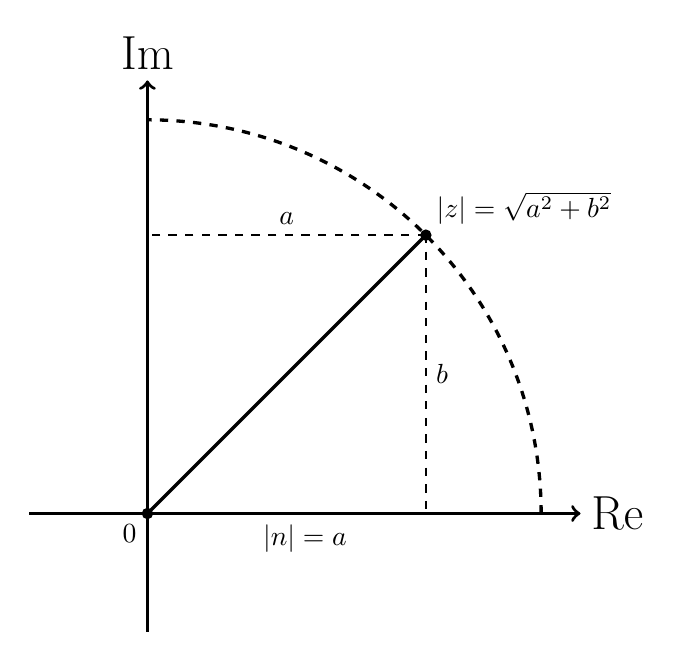
\begin{tikzpicture}

% Define the radius
\def\radius{5}
\def\angle{45} % Angle in degrees

% Convert angle to radians for cos and sin functions
\pgfmathsetmacro\x{\radius * cos(\angle)}
\pgfmathsetmacro\y{\radius * sin(\angle)}

% Draw axes
\draw[very thick, ->] (-1.5,0) -- (\radius+0.5,0) node[right] {\LARGE Re} node[midway, below] {$|n| = a$};
\draw[very thick, ->] (0,-1.5) -- (0,\radius+0.5) node[above] {\LARGE Im};

% Draw complex number
\coordinate (A) at (\x,\y);
\draw[very thick, fill] (A) circle [radius=0.05] node[above right] {$|z| = \sqrt{a^2 + b^2}$};

% Draw origin
\coordinate (O) at (0,0);
\draw[very thick, fill] (O) circle [radius=0.05] node[below left] {$0$};

% Draw line from origin to complex number
\draw[-, very thick] (O) -- (A) node[midway,above, sloped]{};

% Draw quarter circle arc
\draw[very thick, dashed] (\radius,0) arc[start angle=0, end angle=90, radius=\radius];

% Draw right-angle triangle
\draw[thick, dashed] (A) -- (\x,0) node[midway, right] {$b$};
\draw[thick, dashed] (A) -- (0,\y) node[midway, above] {$a$};

\end{tikzpicture}
